\documentclass{article}

\usepackage{graphicx}
\usepackage{tikz}
\usepackage{tikzsymbols}
\usetikzlibrary{calc,patterns,shapes.geometric}
\pagestyle{empty}
\usepackage[margin=0pt]{geometry}
\geometry{papersize={14in,12in}}

\def\centerarc[#1](#2)(#3:#4:#5){\draw[#1] ($(#2)+({#5*cos(#3)},{#5*sin(#3)})$) arc (#3:#4:#5);}

\begin{document}
	\begin{figure}
		\centering
		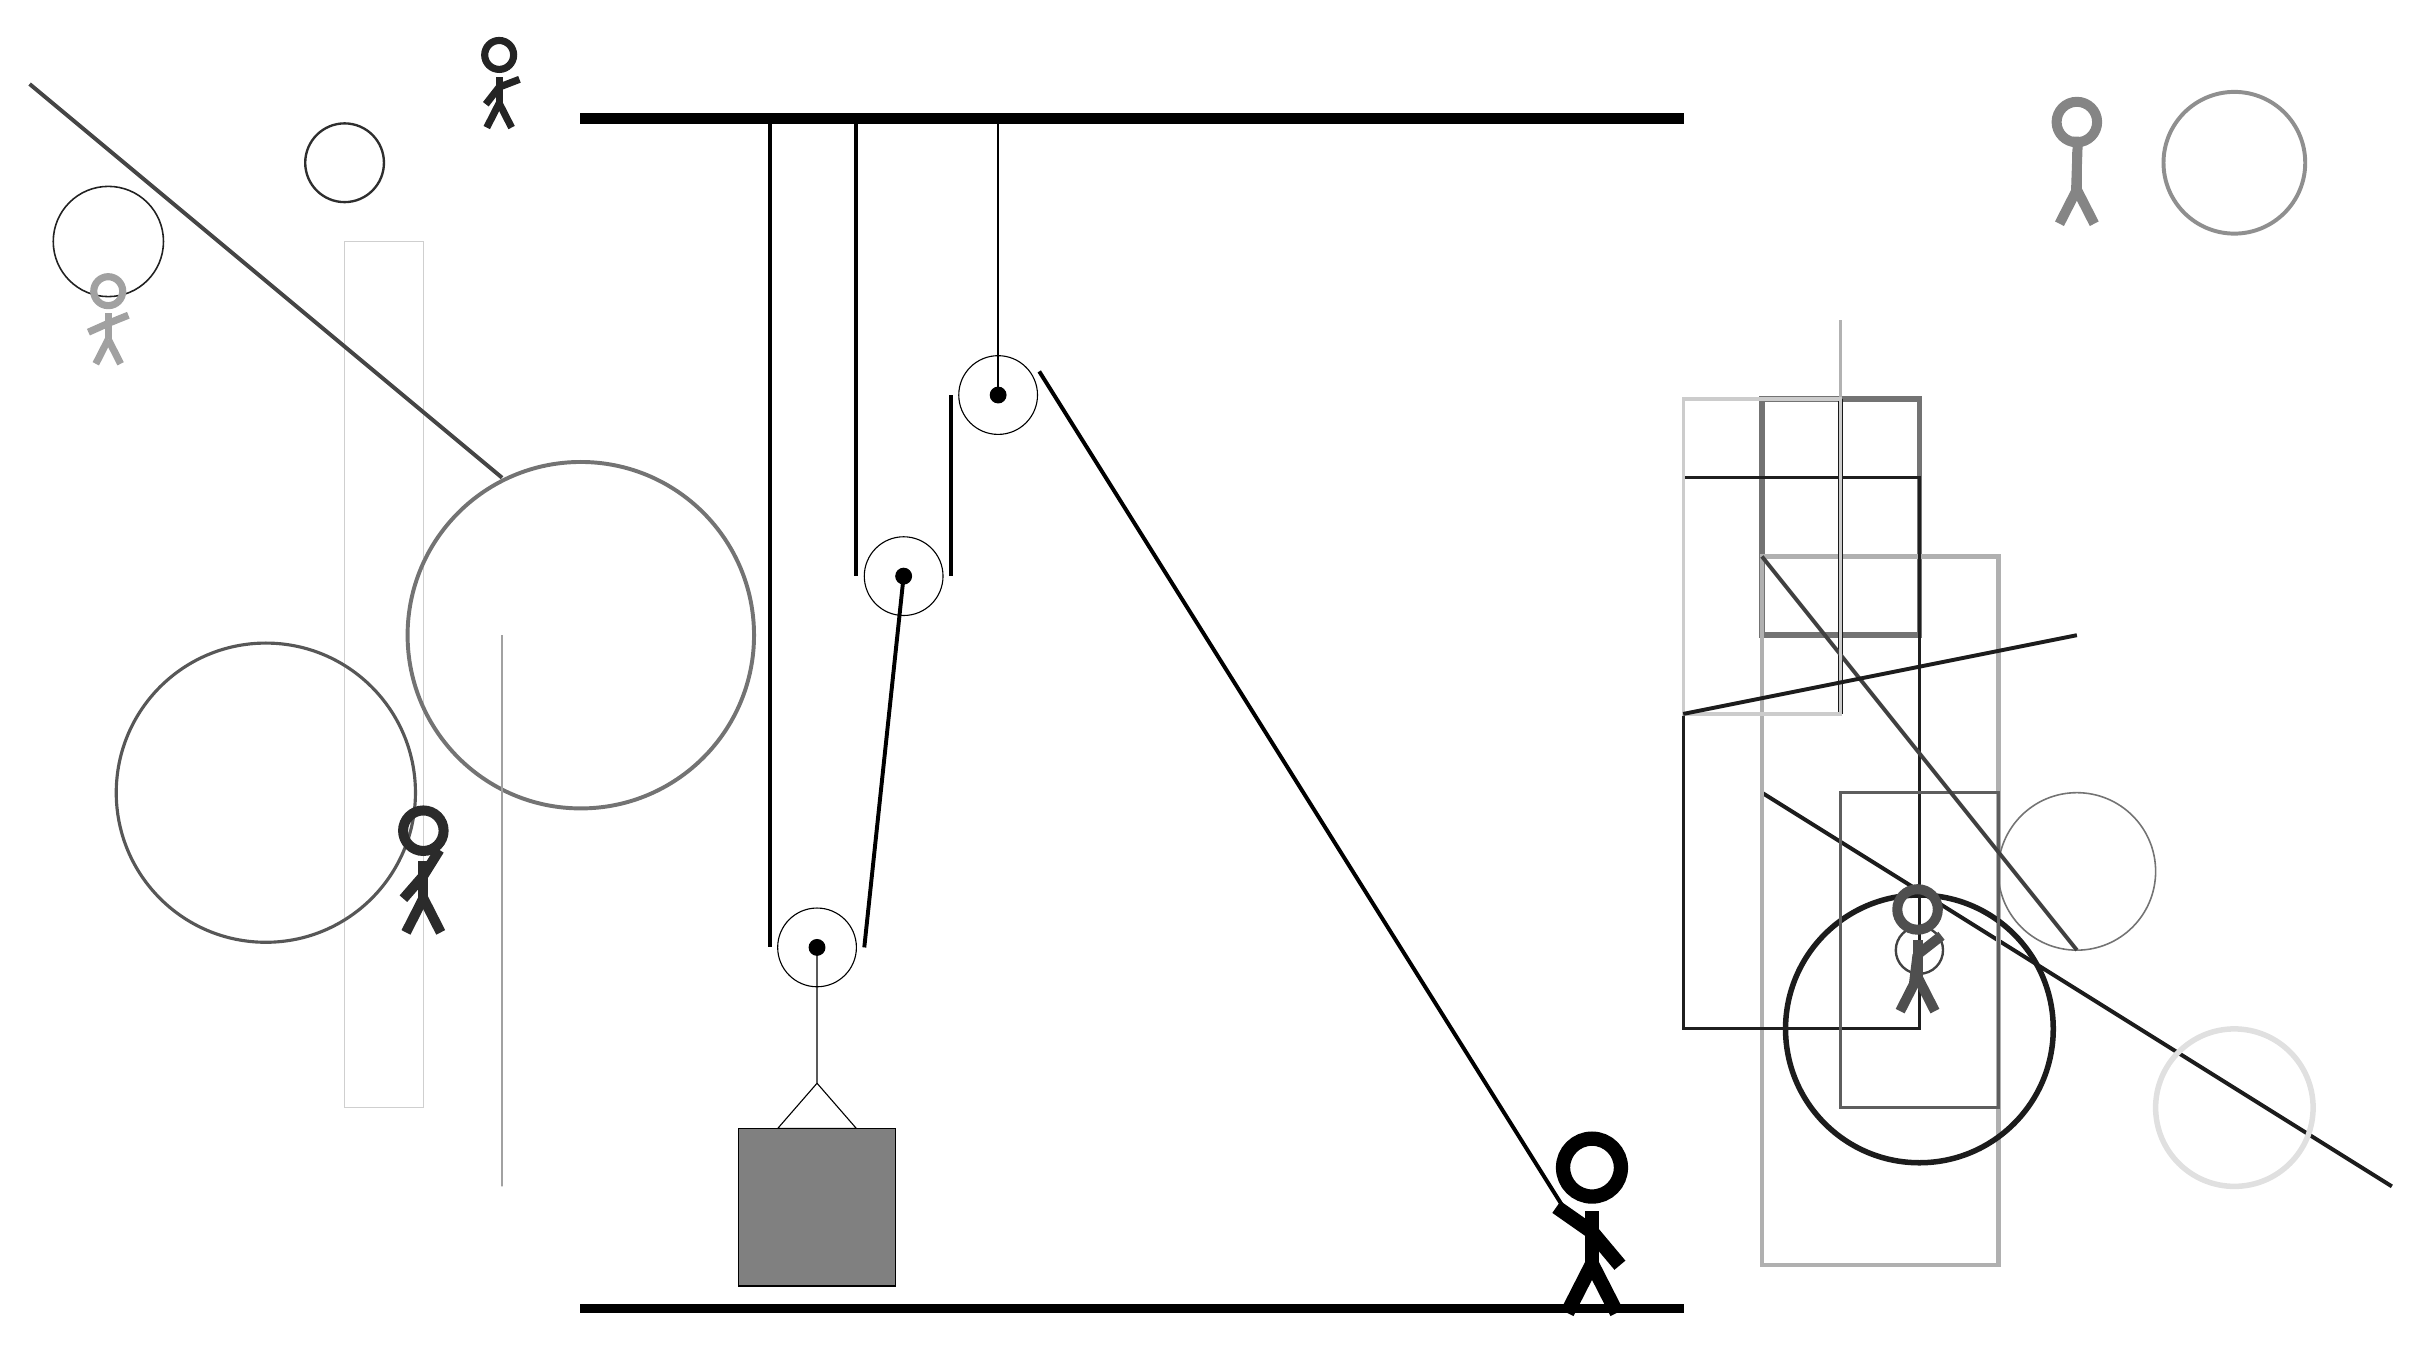
\begin{tikzpicture}
			%%%%% START %%%%%
			
			\draw[fill=black] (-2, 11.5) rectangle (12, 11.625);
			
			\draw (1, 1.035) circle (0.5);
			\draw[fill=black] (1, 1.035) circle (0.1);
			
			\draw (2.1, 5.75) circle (0.5);
			\draw[fill=black] (2.1, 5.75) circle (0.1);
			
			\draw (3.3, 8.05) circle (0.5);
			\draw[fill=black] (3.3, 8.05) circle (0.1);
			\draw[thick] (3.3, 8.05) -- (3.3, 11.5);
			
			\draw (1, 1.035) -- (1, -0.69) -- (0.5, -1.265) -- (1.5, -1.265) -- (1, -0.69);
			\draw[fill=black!50] (0, -1.265) rectangle (2, -3.265);
			
			\draw[line width=0.5mm] (0.4, 11.5) -- (0.4, 1.035);
			\centerarc[line width=0.5mm](1, 1.035)(180:360:0.6);
			\draw[line width=0.5mm](1.6, 1.035) -- (2.1, 5.75);
			\draw[line width=0.5mm] (1.5, 11.5) -- (1.5, 5.75);
			\centerarc[line width=0.5mm](2.1, 5.75)(180:360:0.6);
			\draw[line width=0.5mm](2.7, 5.75) -- (2.7, 8.05);
			\centerarc[line width=0.5mm](3.3, 8.05)(30:180:0.6);
			\draw[line width=0.5mm] (3.822, 8.35) -- (10.5, -2.3);
			
			\node at (10.8, -2.5) {\Strichmaxerl[10][-35][-50]};
			
			\draw [line width=0.2mm, color=black!87](-8, 10) circle (0.7);
			
			\draw[line width=0.2mm, color=black!19] (-4, -1) rectangle (-5, 10);
			\draw[line width=0.5mm, color=black!89](13, 3) -- (21, -2);
			\draw [line width=0.4mm, color=black!66](-6, 3) circle (1.9);
			
			\node[line width=0.5mm, color=black!83] at (-4, 2) {\Strichmaxerl[7][49][58]};
			
			\draw[line width=0.7mm, color=black!55] (13, 5) rectangle (15, 8);
			\draw[line width=0.6mm, color=black!31] (13, 6) rectangle (16, -3);
			\draw[line width=0.6mm, color=black!90] (14, 8) rectangle (14, 4);
			\draw [line width=0.7mm, color=black!89](15, 0) circle (1.7);
			
			\draw [line width=0.5mm, color=black!44](19, 11) circle (0.9);
			\draw[line width=0.4mm, color=black!88] (12, 0) rectangle (15, 7);
			\draw [line width=0.3mm, color=black!74](15, 1) circle (0.3);
			\node[line width=0.3mm, color=black!86] at (-3, 12) {\Strichmaxerl[5][52][21]};
			
			\draw [line width=0.5mm, color=black!55](-2, 5) circle (2.2);
			\node[line width=0.7mm, color=black!69] at (15, 1) {\Strichmaxerl[7][83][38]};
			\node[line width=0.4mm, color=black!37] at (-8, 9) {\Strichmaxerl[5][24][22]};
			
			\draw [line width=0.2mm, color=black!55](17, 2) circle (1.0);
			
			\draw[line width=0.5mm, color=black!73](-3, 7) -- (-9, 12);
			\draw [line width=0.7mm, color=black!12](19, -1) circle (1.0);
			
			\node[line width=0.7mm, color=black!48] at (17, 11) {\Strichmaxerl[7][88][88]};
			\draw[line width=0.4mm, color=black!63] (14, -1) rectangle (16, 3);
			\draw [line width=0.3mm, color=black!82](-5, 11) circle (0.5);
			
			\draw[line width=0.4mm, color=black!30] (14, 8) rectangle (14, 9);
			\draw[line width=0.5mm, color=black!75](13, 6) -- (17, 1);
			\draw[line width=0.4mm, color=black!20] (14, 4) rectangle (12, 8);
			
			\draw[line width=0.5mm, color=black!89](12, 4) -- (17, 5);
			
			\draw[line width=0.3mm, color=black!37] (-3, -2) rectangle (-3, 5);
			
			\draw[fill=black] (-2, -3.5) rectangle (12, -3.6);
			
			%%%%% END %%%%%
		\end{tikzpicture}
	\end{figure}	
\end{document}